\scanpage{30}
\reversemarginpar
\margin{\handwritten{SGA 4 $\overline{\text{\uline{XVI}}}$}}
\normalmarginpar
\mspage{VII 2}

Du point de vue substance, 2.1.1 se ramène trivialement au cas où dans $X\handwritten{\longrightarrow}S$, $X$ est affine, donc quasi-compact quasi-séparé (on dit maintenant ``cohérent''), et alors c'est une conséquence du th. de changement de base par $f$, qui est donné dans SGA \unsure{\deleted{V}4|\deleted{4}V} XVI 1.1\inserted{et qui est essentiellement}. Mais dans loc. cit. on utilise toute la force du théorème de changement de base propre, ce qui est en effet abusif, car en interprétant comme un énoncé d'acyclicité globale 2.1.1, on est ramené comme tu l'observes \deleted{à 2.1.5} au cas particulier 2.1.5, qui se ramène trivialement à son tour au cas du degré de transcendance 1, et par là au th.\unsure{\handwritten{,}} de changement de\inserted{corps de} base pour le $H^1$ premier à $p$ pour une courbe propre et lisse. Je pense présenter les choses ainsi en réédition de SGA 4, de sorte que ton 2.1.1 y sera énoncé en toutes lettres, s'il ne l'est déjà (je n'ai pas les textes en main).
\reversemarginpar
\margin{\figure{\handwritten{\begin{tikzpicture}[x=.012cm,y=.012cm]
\draw[line width=.25pt] (0,0) .. controls (30,-8) and (43,-7) .. (63,12) .. controls (77,27) and (89,43) .. (97,54);
\end{tikzpicture}}}}
\normalmarginpar
Cela te dispensera donc de le prouver, ta seule tâche consistant à interpréter en termes de champs cet énoncé \deleted{(que tu pourrais donner sous forme de rappels)}.

Du point de vue rédaction, on a l'impression que tu t'es ingénié à tout présenter à l'\unsure{\(\mathbb{e}\)|\deleted{E}e|\deleted{e}E}nvers. Il faut en tous cas bloquer ensemble 2.1.1 et 2.1.7 (pratiquement identiques) et 2.1.5 (celui-ci en corollaire, peut-être)
% The following connected cancellation is drawn in its observed geometry.
% Its source origin is approximately (225,1507). The semantic state macros
% retain the cancelled/underlined text; their automatic lines are suppressed
% locally because the actual border, obliques and underlines are drawn below.
% BEGIN cancellation graphic
\begingroup
\renewcommand{\ULthickness}{0pt}
\figure{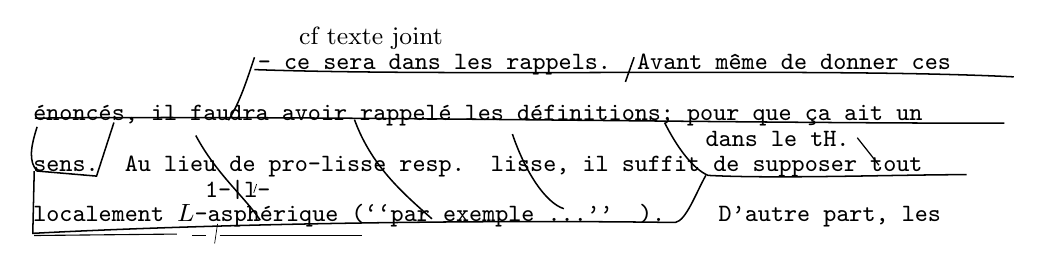
\begin{tikzpicture}[x=.0092cm,y=-.0092cm,every node/.style={inner sep=0pt,anchor=base west,font=\small\ttfamily}]
\node at (310,0) {\deleted{- ce sera dans les rappels\unsure{.} Avant même de donner ces}};
\node[font=\small] at (367,-34) {\inserted{\handwritten{cf texte joint}}};
\node at (0,70) {\deleted{énoncés, il faudra avoir rappelé les définitions; pour que ça ait un}};
\node at (0,140) {\deleted{sens. Au lieu de pro-lisse resp. lisse, il suffit de supposer tout}};
\node at (928,106) {\deleted{\inserted{dans le tH.}}};
\node at (237,177) {\deleted{\inserted{\unsure{1-|l-}}}};
\node at (0,210) {\deleted{\uline{localement} \uline{$L$}-\uline{asphérique} (``par exemple ...'' )}.};
\node at (946,210) {D'autre part, {\renewcommand{\ULthickness}{.4pt}\deleted{les}}};
\draw[line width=.55pt] (306,-17) .. controls (296,13) and (286,45) .. (270,70);
\draw[line width=.55pt] (306,0) .. controls (590,10) and (1090,-3) .. (1354,10);
\draw[line width=.55pt] (830,-17)--(818,17);
\draw[line width=.55pt] (3,67) .. controls (368,63) and (941,74) .. (1341,74);
\draw[line width=.55pt] (6,79) .. controls (-3,107) and (-6,127) .. (6,140)--(88,147)--(112,73);
\draw[line width=.55pt] (2,140)--(0,226) .. controls (247,213) and (600,207) .. (887,211) .. controls (902,208) and (915,171) .. (929,146);
\draw[line width=.55pt] (225,91) .. controls (254,145) and (293,176) .. (314,208);
\draw[line width=.55pt] (444,69) .. controls (467,132) and (509,169) .. (551,206);
\draw[line width=.55pt] (662,89) .. controls (680,142) and (708,184) .. (733,192);
\draw[line width=.55pt] (872,73) .. controls (889,107) and (911,137) .. (932,146) .. controls (1027,151) and (1191,145) .. (1289,145);
\draw[line width=.45pt] (1138,94)--(1168,132);
\draw[line width=.4pt] (2,229)--(199,227);
\draw[line width=.4pt] (220,229)--(239,229);
\draw[line width=.4pt] (258,229)--(454,229);
\draw[line width=.25pt] (309,158)--(305,170);
\draw[line width=.25pt] (255,213)--(251,240);
\end{tikzpicture}}
\endgroup
% END cancellation graphic
\reversemarginpar
\margin{\handwritten{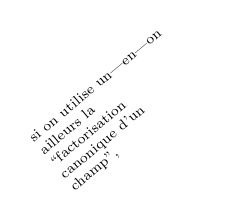
\begin{tikzpicture}[scale=.72,transform shape]
\node[rotate=40,anchor=south west,align=left,inner sep=0pt,font=\scriptsize] at (0,0) {\unsure{si on utilise} \unsure{un|en|on}\\ailleurs la\\``factorisation\\\unsure{c}anonique d'un\\champ'',};
\end{tikzpicture}}}
\normalmarginpar
\deleted{énoncés} 2.12, 2.1.3, 2.1.4, 2.1.7.1 n'ont rien à voir avec les schémas, il sont manifestement importants en eux-mêmes et devraient passer dans un numéro à part dans
% BEGIN reference correction
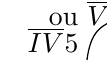
\begin{tikzpicture}[baseline=(iv.base),x=.01cm,y=.01cm]
\node[inner sep=0pt,anchor=base west] (iv) at (0,0) {\handwritten{$\overline{\text{\uline{IV}}}$}};
\node[inner sep=0pt,anchor=base west] at (47,0) {\deleted{5}};
\node[overlay,inner sep=0pt,anchor=base west] at (27,34) {\inserted{\handwritten{ou $\overline{\text{\uline{V}}}$}}};
\draw[overlay,line width=.45pt] (76,-10) .. controls (81,26) and (92,36) .. (126,45) .. controls (143,51) and (150,57) .. (152,65);
\end{tikzpicture}
% END reference correction
(avec un peu d'ordre dans la suite des énoncés)

% BEGIN final cancelled line
\figure{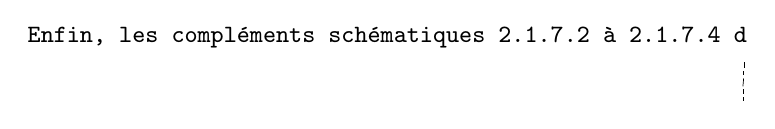
\begin{tikzpicture}[x=.0092cm,y=-.0092cm]
\node[inner sep=0pt,anchor=base west,font=\small\ttfamily] at (0,0) {\deleted{Enfin, les compléments schématiques 2.1.7.2 à 2.1.7.4 d}};
\draw[line width=.25pt] (990,27)--(990,34);
\draw[line width=.25pt] (989,39)--(989,45);
\draw[line width=.25pt] (989,49)--(988,60);
\draw[line width=.25pt] (988,64)--(988,70);
\draw[line width=.25pt] (988,75)--(988,80);
\end{tikzpicture}}
% END final cancelled line
% archive sheet number: 29
